\section{Aprendizado de máquina}

Aprendizado pode ser definido como qualquer mudança em um sistema que
otimize o seu desempenho na segunda vez que ele repetir a mesma tarefa,
ou outra tarefa da mesma população~\cite{custodio2010aprendizadomaquina}.

O aprendizado de máquina utiliza um princípio de inferência denominado
indução, onde através de um conjunto particular de exemplos é possível
obter conclusões genéricas~\cite{bruno2010aprendizadomaquina}. De um modo
abstrato o aprendizado de máquina funciona como uma caixa preta, onde
independente de como é implementado, o mesmo deve ser capaz de encontrar padrões
nos dados apresentados e criar um modelo para dados que ainda não foram vistos.

Como exemplo, o aprendizado de máquina pode ser usado para classifcar
um conjunto de atributos. Exemplo assim são bastante comuns quando se fala em
aprendizado de máquina. \citeonline{lecun1989backpropagation} usou algoritmos de
aprendizado de máquina para classificar códigos postais escritos a mão. Outro
exemplo está no trabalho de \citeonline{stallkamp2012man}, que usa método de
aprendizado de máquina para classificar placas de trânsito em diferentes
condições.


\subsection{Aprendizado supervisionado}

Quando se fala de aprendizado de máquina, várias técnicas distintas podem ser
usadas, entretanto, uma das principais técnicas de aprendizado de máquina é o aprendizado
supervisionado, onde é fornecido um treinamento com o conhecimento do
ambiente, que é composto por um conjunto de exemplos com entradas
e uma saída esperada~\cite{bruno2010aprendizadomaquina}.

O objetivo do aprendizado supervisionado é induzir conceitos a partir de
exemplos que estão pré-classificados, em outras palavras, exemplos que
possuem um rótulo associado a uma classe conhecida~\cite{bruno2010aprendizadomaquina}.
Utilizado quando se tem tanto as perguntas quanto as respostas, o aprendizado
supervisionado é utilizado para se obter uma classificação e funções de aproximação, ou seja,
tais algoritmos produzem um modelo à partir de dados já classificados capaz de estimar classificações
para dados ainda não vistos.

Utilizando do exemplo do algoritmo que classifica um conjunto de atributos,
na utilização do aprendizado supervisionado, para cada entrada do treinamento
existe um rótulo, que se trata da classificação do conjunto de atributos, ou
seja, apenas possui os valores 0, 1 e 2, entrada também possui os valores dos
atributos associados ao rótulo. A tabela~\ref{tab:entradas_de_treinamento}
mostra um exemplo das entradas de treinamento.

\begin{table}[h]
\centering
\resizebox{\textwidth}{!}{\begin{tabular}{|l|l|l|l|l|l|}
\hline
\rowcolor[HTML]{EFEFEF}
{\textbf{Rótulo}} & {\textbf{Atributo 1}} & {\textbf{Atributo 2}} & {\textbf{Atributo 3}} & {\textbf{Atributo 4}} & {\textbf{Atributo 5}} \\ \hline
1 & 1 & 0 & 1 & 0 & 1 \\
\hline
2 & 0 & 1 & 1 & 0 & 1 \\
\hline
0 & 1 & 0 & 0 & 1 & 1 \\
\hline
1 & 1 & 0 & 1 & 1 & 0 \\
\hline
2 & 0 & 1 & 1 & 1 & 0 \\
\hline
\end{tabular}}
\caption{Entradas de treinamento para o aprendizado de máquina}
\label{tab:entradas_de_treinamento}
\end{table}

Após ser realizada a etapa de treinamento, ao receber uma sequencia de cinco
atributos, o algoritmo deve retornar qual o rótulo, ou seja, a classificação,
correspondente a esses atributos. A tabela~\ref{tab:entrada_para_classificar}
mostra um exemplo de entrada para o algoritmo, a diferença dessa entrada para
a de treinamento é que essa não possui o rótulo, pois o rótulo será o resultado
da execução do algoritmo.

\begin{table}[h]
\centering
\resizebox{\textwidth}{!}{\begin{tabular}{|l|l|l|l|l|}
\hline
\rowcolor[HTML]{EFEFEF}
{\textbf{Atributo 1}} & {\textbf{Atributo 2}} & {\textbf{Atributo 3}} & {\textbf{Atributo 4}} & {\textbf{Atributo 5}} \\ \hline
1 & 0 & 1 & 1 & 0 \\
\hline
\end{tabular}}
\caption{Entrada de dados para o algoritmo determinar o rótulo}
\label{tab:entrada_para_classificar}
\end{table}


\subsection{Classificador Bayesiano} \label{sec:classificador_bayesiano}

Uma técnica famosa de algoritmos supervisionados é o classificador bayesiano,
que é normalmente chamado de \textit{naive bayes}. Esse algoritmo é baseado no
princípio da probabilidade bayesiana, entretanto, diferente do modelo em si,
ele admite que os atributos de um dado são sempre independentes um do outro,
mesmo que os atributos possuam alguma dependência um do outro \cite{segaran2007programming}

Sendo assim, o classificador bayesiano irá basicamente classificar um dado
como pertencente a uma classe, se tal classe obter o maior valor de
probabilidade dentre os valores de classe possíveis. Dessa forma, pode-se
dizer que a classificação bayesiana segue o seguinte formato:

$Classificador = max(p(C_{y})*\prod_{i=1}^{N}p(x_{i}|C_{y}))$

Onde:

\begin{itemize}
    \item \textbf{$C_{y}$: } Uma das classes possíveis para classificar um
    dado;
    \item \textbf{n: } Número total de itens;
    \item \textbf{$p(C_{y})$: } Probabilidade da classe ``y'' dentro do
    conjunto de dados. Pode ser calculado pela
    fórmula: $\frac{NC_{y}}{N_{t}}$.
    Onde:
      \begin{itemize}
          \item \textbf{$NC_{y}$: } Número de itens da classe ''y'';
          \item \textbf{$N_{t}$: } Número total de classes;
      \end{itemize}
    \item \textbf{$p(x_{i}|C_{y})$: } Cálculo da probabilidade bayesiana
    em si, assumindo que as variáveis são independentes. Tal expressão
    pode ser calculada pela seguinte fórmula: $\frac{Nxi_{C_{y}}}{NC_{y}}$.
    Onde $Nxi_{C_{y}}$ é o número de vezes que o atributo $x_{i}$ aparece
    dentro de um dado marcado como $C_{y}$.
\end{itemize}

Dessa forma, pode-se ver o modelo gerado por esse algoritmo supervisionado
é nada mais com que as probabilidades $p(C_{y})$ e $p(x_{i}|C_{y})$ para
todas as possíveis classificações que serão usadas no problema. Dessa forma,
os dados usados para alimentar tal algoritmo são para criar exatamente tais
dados. Uma vez com eles calculados, o modelo do algoritmo está completo,
podendo o mesmo ser usado para classificar dados ainda não vistos.

Vale ressaltar que o modelo apresentado tem como base a classificação
bayesiana usando o modelo de Bernoulli, onde os valores de $x_{i}$ são valores
binários, indicando assim a presença ou não de um atributo em um certo dado.
Para valores discretos, pode-se usar outros modelos, como o Gaussiano, onde
seria necessário o cálculo da média e variância dos atributos para as dadas
classes de classificação \cite{zhang2004optimality}.

Apesar da simplicidade desse algoritmo, alguns cuidados devem ser observados.
O primeiro cuidado é analisar as variáveis, pois quando estas possuem uma grande
dependência entre elas, pode levar o modelo a acarretar problemas. O outro cuidado
se dá no uso dos atributos que são usados para gerar a classificação de um dado.
Apesar dessa preocupação estar presente em algoritmos supervisionados em geral,
o número de cálculos necessários para esse sistema aumenta consideravelmente a
cada novo atributo adicionado, podendo assim ocasionar problemas de performance.

\subsection{Engenharia de atributos}

Considerando que o aprendizado de máquina tem como um alicerce os dados de entrada
e principalmente as características desses dados, deve-se ter um cuidado
significativo ao selecionar os atributos que serão usados para alimentar um
algoritmo de aprendizado de máquina. Essa problemática se torna ainda maior
quando um dado apresentado possui um conjunto de atributos muito grande, ou
seja, possui uma dimensão alta. Quando isso acontece, pode-se dizer que a
densidade entre os dados e as distâncias entre os mesmos se tornam menos
significativas \cite{amatriain2011data}. Esse efeito se chama \textit{maldição
da dimensionalidade} e pode afetar negativamente um série de algoritmos de
aprendizado de máquina.

Um dos efeitos diretos desse problema é o caso chamado de \textit{overfitting}.
Esse problema acontece quando um algoritmo fica viciado nas entradas na qual foi
treinado e não apresenta resultados satisfatórios quando recebe dados desconhecidos.
Sendo assim, uma das formas de evitar tal problema é selecionar bem os atributos
de um projeto ou até mesmo usar técnicas para diminuir a dimensionalidade de uma
variável de entrada.

Caso a seleção seja manual, é recomendável que a mesma seja realizada ao lado de
um especialista na área na qual o aprendizado de máquina será utilizado. Isso se
dá pela capacidade de um profissional da área em informar que atributos são
relevantes para a classicação de um determindado objeto.

O segundo método se dá pelo uso de técnicas computacionais para reduzir a
dimensão de uma variável. Um exemplo dessa técnica é o \textit{Principal
Component Analysis (PCA) } que ordena os atributos que maior contribuem para a
variância dos dados em relação ao método de mínimos quadrados
\cite{amatriain2011data}. Normalmente, tal método ignora atributos após a
variãncia acumulada passar de 90\%.

Apesar da aplicação de ambas as formas em conjunto serem possíveis, vale lembrar
que ambas possuem limitações. Para a seleção manual de atributos, pode-se ter
casos onde a classificação dos dados nunca foi feita ou até mesmo a dificuldade
em se encontrar um especialista na área para ajudar na seleção. Enquanto isso,
para algoritmos de redução, algumas limitações também existem. Para o caso do
PCA, o mesmo parte do pressuposto que os dados apresentados seguem uma
distribuição Gaussiana. Quando isso não acorre, nada pode-se garantir quanto a
seleção dos atributos mais significativos \cite{amatriain2011data}. Mesmo com
essas dificuldades, essa etapa é crucial para um bom funcionamento do algoritmo
de aprendizado de máquina, principalmente quanto a escalabilidade do mesmo.


\subsection{Validação cruzada}

Uma das formas de validar se o algoritmo não está sofrendo \textit{overfitting}
e o seu oposto, \textit{underfitting}, onde o algoritmo apresenta elevado valor
de \textit{bias} para as entradas usadas como teste, ou seja, o modelo criado
pelo algoritmo é muito simples. Uma forma de observar a ocorrência desses dois
fenômenos é pela técnica estatística de validação cruzada. Essa técnica é
comumente usada para avaliar modelos preditivos, e se baseia na separação dos
dados existentes em uma parte de treinamento e uma parte de teste. A conjunto de
dados de treinamento é usado para alimentar o algoritmo. Após o treinamento,
e o conjunto de teste é então usado para validar o algoritmo. \cite{araujo2011apprecommender}.

Uma forma de tornar o processo de validação cruzada visual é o uso de curvas de
aprendizado. Uma curva de aprendizado pode ser vista como a relação das curvas
erro do conjunto de dados de treinamento e a curva dos dados de teste. Isso pode
ser visto como melhor foco na Figura \ref{fig:curva_aprendizado}.

\begin{figure}[h]
  \centering
  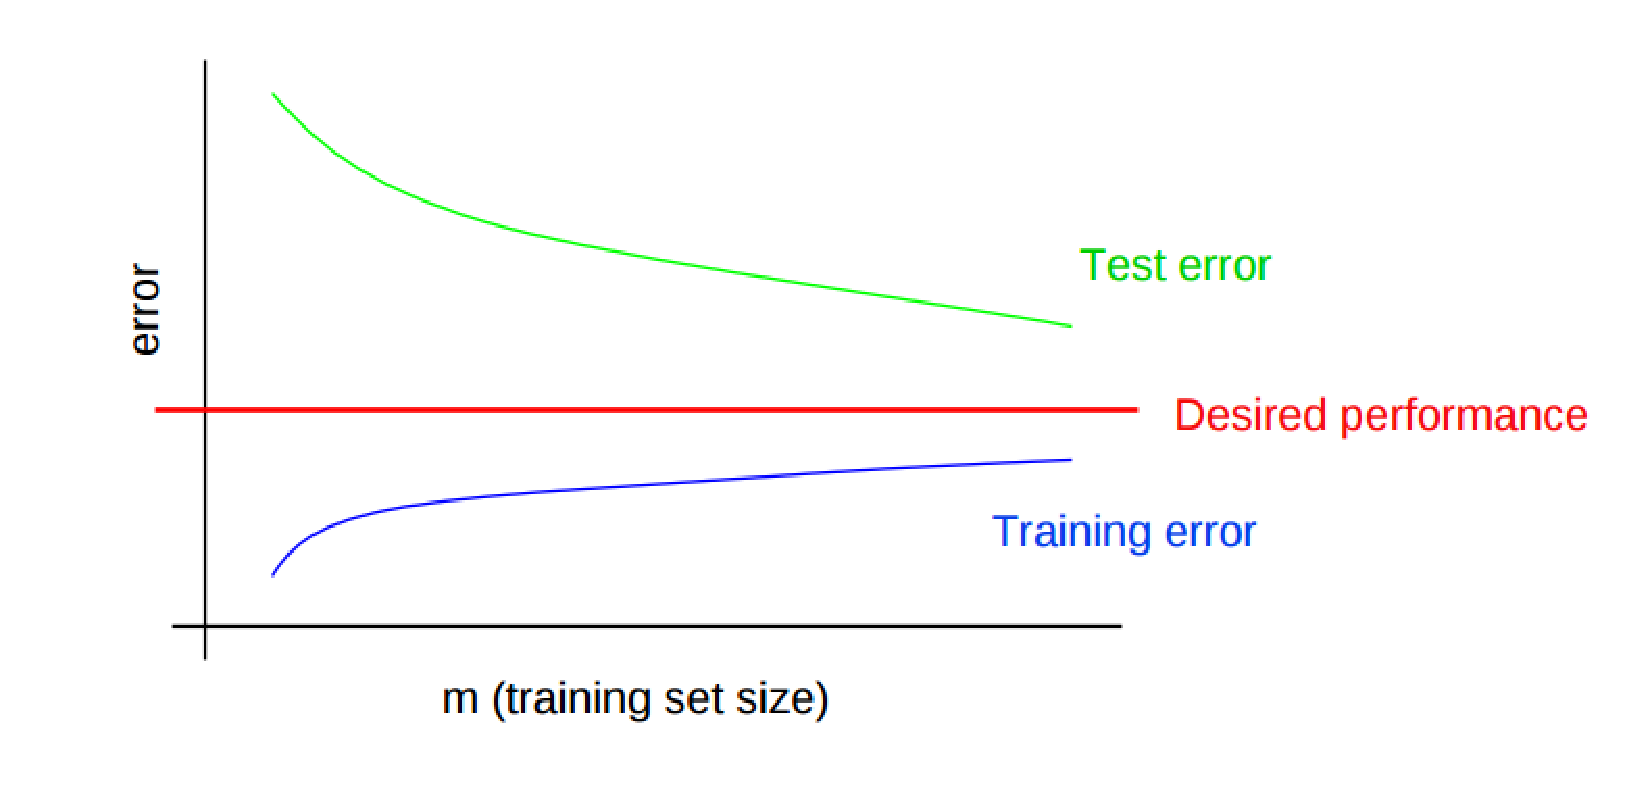
\includegraphics[width=0.9\textwidth]{figuras/curva_aprendizado.eps}
  \caption{Exemplo de uma curva de aprendizado \cite{1_ng} }
  \label{fig:curva_aprendizado}
\end{figure}

Pode-se ver na figura \ref{fig:curva_aprendizado}, o eixo das ordenadas representa
o valor do erro, enquanto o eixo das abscissas representa o tamanho do conjunto de
dado usado para treinamento. Para calcular o erro apresentado nos gráficos, pode-se
usar qualquer fórmula estatística para tal fim. Entretanto, uma das mais comuns
quando se trata de validação cruzada é a seguinte \cite{1_ng}:

\begin{equation}
ErroTreinamento = \frac{1}{2m}*\sum_{i=0}^{m}(h(x_{i}) - y(x_{i}))^2
\end{equation}

\begin{equation}
ErroTeste = \frac{1}{2m_{teste}}*\sum_{i=0}^{m_{teste}}(h(x_{t}^{i}) - y(x_{t}^{i}))^2
\end{equation}

Onde:

\begin{itemize}
    \item \textbf{m: } Tamanho do conjunto de teste;
    \item \textbf{$h(x_{i}$): } Função que reflete o modelo criado por um algoritmo
    de aprendizado de máquina, ou seja, recebe um dado e retorna um classificação.
    \item \textbf{$y(x): $} Valore real da classificação para o dado sendo apresentado
    \item \textbf{$m_{teste}$: } Tamanho do conjunto de teste obtido por validação cruzada.
\end{itemize}

Dessa forma, pode-se ver que o gráfico mostra a evolução do modelo produzido pelos
dados de treinamento em relação ao conjunto de dados obtidos pela validação cruzada,
variando-se o número de dados usados no treinamento. É esperado que inicialmente, as
curvas fiquem bem distantes uma da outra, pois com poucos dados de treinamento, o
conjunto de teste apresentára erros altos, enquanto o conjunto de treinamento não.
Entrentanto, com mais dados de treinamento usados, é esperado que as curvas se
aproximem mais uma da outra.

O uso desses gráficos pode-se bastante útil para encontrar casos de \textit{overfitting}
e \textit{underfitting} pois tais casos podem ser claramente identificados observando-se
o gráfico. Em um conjunto de teste onde ao final, as curvas de treinamento e de erro estão
muito distantes, pode-se entender que o algoritmo está apresentando \textit{underfitting}.
Entretanto, caso as curvas estejam muito próximas quando se usa todos os dados de
treinamento alocados, pode-se entender uma baixa variância do modelo, identificando assim
um caso de \textit{overfitting}.

\subsection{Bayes Ingênuo}

Dado o contexto do classificador bayesiano apresentado na seção
\ref{sec:classificador_bayesiano}, resolveu-se implementar tais fórmulas usando
apenas manipulação de matrizes. Essa decisão se deu principalmente por questões
de performance, principalmente pelo fato de que o perfil do usuário pode mudar
com alta frequência, necessitando que o treinamento do algoritmo seja eficaz.

Para mostrar o modelo criado, a tabela \ref{tab:entradas_de_treinamento} será
usada. Primeiramente, esta tabela será dividida em duas matrizes distintas, D e
L. A matriz D representa os atributos de cada item. Dessa forma, sua dimensão
será ``${e \times a}$'', onde ``e'' é significa os número de itens na tabela, e
``a'' representa o número de atributos que cada item possui. Já a matriz L
representa a classificação para cada item ``e'' encontrado na matriz D. Dessa
forma, a mesma será uma matriz coluna com dimensão ``${e \times 1}$''.

$$D=\left[
\begin{array}{ccccc}
1 & 0 & 1 & 0 & 1 \\
0 & 1 & 1 & 0 & 1 \\
1 & 0 & 0 & 1 & 1 \\
1 & 0 & 1 & 1 & 0 \\
0 & 1 & 1 & 1 & 0 \\
\end{array}
\right]_{e \times a}$$

$$L=\left[
\begin{array}{c}
1 \\
2 \\
0 \\
1 \\
2 \\
\end{array}
\right]_{e \times 1}$$

Para o algoritmo funcionar também é necessário ter conhecimento de quais são as
classificações possíveis, essas classificações são informadas
através do vetor coluna B, com dimensões ``${l \times 1}$'', onde ``l'' é o número
de classificações possíveis.

$$B=\left[
\begin{array}{c}
0 \\
1 \\
2 \\
\end{array}
\right]_{l \times 1}$$

Utilizando a matriz D e os vetores L e B, monta-se a matriz de adjacência A, onde
cada linha dessa matriz representa respectivamente um classificação possível, e cada
coluna da matriz identifica se um item da matriz D foi classificado de acordo
com a classificação representada pela linha em que se encontra. A matriz de adjacência A também é uma
matriz com valores binários, onde ``1'' indica a presença do item na classificação,
e ``0'' indica a ausência do item na classificação. Logo a matriz A possui
dimensões ``${l \times e}$''.

$$A=\left[
\begin{array}{ccccc}
0 & 0 & 1 & 0 & 0 \\
1 & 0 & 0 & 1 & 0 \\
0 & 1 & 0 & 0 & 1 \\
\end{array}
\right]_{l \times e}$$

Utilizando a matriz A pode-se calcular o vetor com o histograma do vetor L, onde
cada linha do vetor histograma H representa uma possível
classificação da matriz B, e o valor de cada coluna representa o número de itens
no qual a classificação está associada. O vetor coluna H é calculado pela multiplicação da matriz A pelo
vetor coluna com todos os valores sendo ``1'', onde esse vetor coluna possui ``e''
linhas, logo as dimensões do vetor coluna H são ``${l \times 1}$''

$$H=A_{l \times e} * \left[
\begin{array}{c}
1 \\
1 \\
1 \\
1 \\
1 \\
\end{array}
\right]_{e \times 1}$$

$$H=\left[
\begin{array}{c}
1 \\
2 \\
2 \\
\end{array}
\right]_{l \times 1}$$

Utilizando o vetor H é calculado a probabilidade de cada classificação, que é representada
pelo vetor PH, resultante da divisão do vetor H por ``e''.

\begin{center}
$PH= \frac{1}{e} * H_{l \times 1}$
\end{center}

$$PH=\left[
\begin{array}{c}
\frac{1}{5} \\
\frac{2}{5} \\
\frac{2}{5} \\
\end{array}
\right]_{l \times 1}$$

O próximo passo é calcular a matriz PR1, que se trata da probabilidade de um
atributo ser igual a ``1'', na relação entre as classificações possíveis, o vetor B, e os
atributos da matriz D. Para isso é necessário identificar quantos atributos
estão presentes em cada uma das classificações possíveis, valor esse  obtido pela multiplicação da matriz A
com a matriz D, resultando na matriz R contendo para cada possível classificação
quantos atributos estão presentes na mesma. Com a matriz R calculada, pode-se
obter a matriz de probabilidade PR1, que é o resultado da multiplicação entre a
matriz inversa da diagonal feita pelo vetor H com a matriz R.

\begin{center}
$R = A_{l \times e} * D_{e \times a}$
\end{center}

$$R=\left[
\begin{array}{ccccc}
1 & 0 & 0 & 1 & 1 \\
2 & 0 & 2 & 1 & 1 \\
0 & 2 & 2 & 1 & 1 \\
\end{array}
\right]_{l \times a}$$

$$diag(H)=\left[
\begin{array}{ccc}
1 & 0 & 0 \\
0 & 2 & 0 \\
0 & 0 & 2 \\
\end{array}
\right]_{l \times l}$$

$$diag(H)^{-1}=\left[
\begin{array}{ccc}
1 & 0 & 0 \\
0 & \frac{1}{2} & 0 \\
0 & 0 & \frac{1}{2} \\
\end{array}
\right]_{l \times l}$$

\begin{center}
$PR1 = diag(H)^{-1}_{l \times l} * R_{l \times a}$
\end{center}

$$PR1=\left[
\begin{array}{ccccc}
1 & 0 & 0 & 1 & 1 \\
1 & 0 & 1 & \frac{1}{2} & \frac{1}{2} \\
0 & 1 & 1 & \frac{1}{2} & \frac{1}{2} \\
\end{array}
\right]_{l \times a}$$

Também é necessário identificar a matriz PR0, que indica a probabilidade dos
atributos possuirem o valor zero, essa matriz pode ser obtida através da
expressão ``$1 - PR1$''.

\begin{center}
$PR0 \ = \ 1 \ - \ PR1_{l \times a}$
\end{center}

$$PR0=\left[
\begin{array}{ccccc}
0 & 1 & 1 & 0 & 0 \\
0 & 1 & 0 & \frac{1}{2} & \frac{1}{2} \\
1 & 0 & 0 & \frac{1}{2} & \frac{1}{2} \\
\end{array}
\right]_{l \times a}$$

É necessário transformar as matrizes PR1 e PR0 em matrizes quadradas,
sendo suas dimensões ``${l \times a}$'', a matriz quadrada deve possuir
a maior dentre as duas dimensões, neste caso as matrizes devem possuir
as dimensões ``${a \times a}$'', para que isso aconteça as matrizes são
multiplicadas pela matriz identidade de dimensões ``${a \times l}$''.

$$PR1=\left[
\begin{array}{ccc}
1 & 0 & 0 \\
0 & 1 & 0 \\
0 & 0 & 1 \\
0 & 0 & 0 \\
0 & 0 & 0 \\
\end{array}
\right]_{a \times l}
\left[
\begin{array}{ccccc}
1 & 0 & 0 & 1 & 1 \\
1 & 0 & 1 & \frac{1}{2} & \frac{1}{2} \\
0 & 1 & 1 & \frac{1}{2} & \frac{1}{2} \\
\end{array}
\right]_{l \times a}
= \left[
\begin{array}{ccccc}
1 & 0 & 0 & 1 & 1 \\
1 & 0 & 1 & \frac{1}{2} & \frac{1}{2} \\
0 & 1 & 1 & \frac{1}{2} & \frac{1}{2} \\
0 & 0 & 0 & 0 & 0 \\
0 & 0 & 0 & 0 & 0 \\
\end{array}
\right]_{a \times a}$$

$$PR0=\left[
\begin{array}{ccc}
1 & 0 & 0 \\
0 & 1 & 0 \\
0 & 0 & 1 \\
0 & 0 & 0 \\
0 & 0 & 0 \\
\end{array}
\right]_{a \times l}
\left[
\begin{array}{ccccc}
0 & 1 & 1 & 0 & 0 \\
0 & 1 & 0 & \frac{1}{2} & \frac{1}{2} \\
1 & 0 & 0 & \frac{1}{2} & \frac{1}{2} \\
\end{array}
\right]_{l \times a}
= \left[
\begin{array}{ccccc}
0 & 1 & 1 & 0 & 0 \\
0 & 1 & 0 & \frac{1}{2} & \frac{1}{2} \\
1 & 0 & 0 & \frac{1}{2} & \frac{1}{2} \\
0 & 0 & 0 & 0 & 0 \\
0 & 0 & 0 & 0 & 0 \\
\end{array}
\right]_{a \times a}$$

Obtendo o vetor PH, que é a probabilidade individual de cada rótulo, e a
matrizes PR1 e PR0, o treinamento do algoritmo está completo.

Com o algoritmo treinado, ele está pronto para receber um vetor com
os atributos, como mostra a tabela~\ref{tab:entrada_para_classificar},
é usado como exemplo o vetor v, que possui dimensões ``${1 \times a}$''.

$$v=\left[
\begin{array}{ccccc}
1 & 0 & 1 & 1 & 0 \\
\end{array}
\right]_{1 \times a}$$

O próximo passo é montar a matriz PV, que se trata da matriz de
probabilidade para o vetor. Essa matriz é criada através da junção das matrizes
PR1 e PR0. Entretanto, esse junção tem relação direta com os valores do vetor v,
pois se uma de suas colunas encontra-se o ``1'', deve-se utilizar a coluna da matriz PR1,
e o contrário, utilliza-se a coluna da matriz PR0. Em outras palavras, a matriz PV é resultante
da soma dos produtos entre PR1 e a matriz diagonal de v, com PR0
e a matriz diagonal de v', onde o vetor v' se trata do vetor v com seus valores
alternados.

$$v'=1-\left[
\begin{array}{ccccc}
1 & 0 & 1 & 1 & 0 \\
\end{array}
\right]_{1 \times a}
=
\left[
\begin{array}{ccccc}
0 & 1 & 0 & 0 & 1 \\
\end{array}
\right]_{1 \times a}
$$
\\

\begin{center}
$PV = PR1_{a \times a} * diagonal(v)_{a \times a} \ + \ PR0_{a \times a} * diagonal(v')_{a \times a}$
\end{center}

$$PV=
\left[
\begin{array}{ccccc}
1 & 0 & 0 & 1 & 1 \\
1 & 0 & 1 & \frac{1}{2} & \frac{1}{2} \\
0 & 1 & 1 & \frac{1}{2} & \frac{1}{2} \\
0 & 0 & 0 & 0 & 0 \\
0 & 0 & 0 & 0 & 0 \\
\end{array}
\right]_{a \times a}
\left[
\begin{array}{ccccc}
1 & 0 & 0 & 0 & 0 \\
0 & 0 & 0 & 0 & 0 \\
0 & 0 & 1 & 0 & 0 \\
0 & 0 & 0 & 1 & 0 \\
0 & 0 & 0 & 0 & 0 \\
\end{array}
\right]_{a \times a}
+
\left[
\begin{array}{ccccc}
0 & 1 & 1 & 0 & 0 \\
0 & 1 & 0 & \frac{1}{2} & \frac{1}{2} \\
1 & 0 & 0 & \frac{1}{2} & \frac{1}{2} \\
0 & 0 & 0 & 0 & 0 \\
0 & 0 & 0 & 0 & 0 \\
\end{array}
\right]_{a \times a}
\left[
\begin{array}{ccccc}
0 & 0 & 0 & 0 & 0 \\
0 & 1 & 0 & 0 & 0 \\
0 & 0 & 0 & 0 & 0 \\
0 & 0 & 0 & 0 & 0 \\
0 & 0 & 0 & 0 & 1 \\
\end{array}
\right]_{a \times a}
$$

$$PV=\left[
\begin{array}{ccccc}
1 & 1 & 0 & 1 & 0 \\
1 & 1 & 1 & \frac{1}{2} & \frac{1}{2} \\
0 & 0 & 1 & \frac{1}{2} & \frac{1}{2} \\
0 & 0 & 0 & 0 & 0 \\
0 & 0 & 0 & 0 & 0 \\
\end{array}
\right]_{a \times a}$$

O próximo passo seria então usar a matriz PV para encontrar classificação que
apresenta maior valor para o vetor v. Antes disso, decidiu-se normatizar todos
os valores de PV pelo função logaritmo. Entretanto, alguns valores de PV podem
possuir o valor ``0'', pois tal valor indica que um determinado atributo para
uma dada classificação não nunca apareceu. Considerando que tal valor não é
definido na função logaritmo, resolveu-se antes somar ``1'' a matriz PV e logo
após calcular calcular a matriz logaritmica dessa nova matriz.

Através da matriz PV é obtido o vetor coluna ``u'', onde cada linha
do vetor u corresponde a multiplicação dos elementos da linha da matriz
PV, porém devido ao fato de uma probabilidade zero em uma linha da matriz
PV irá fazer com que a multiplicação da linha seja igual a zero, para
impedir esse problema é somado 1 a matriz PV. Como a matriz pode ter
centenas de atributos ``a'' existe o problema de que a multiplicação
desses elementos tornem a multiplicação das linhas da matriz um número
muito grande, ou um número muito pequeno, afim de impedir que ocorra
problemas computacionais com o tamanho dos números, ao invés de multiplicar
as linhas da matriz, é somado o log de cada elemento da matriz PV resultando
no vetor ``u''.

\begin{center}
$PV = PV_{a \times a} + 1$
$$PV=\left[
\begin{array}{ccccc}
2 & 2 & 1 & 2 & 1 \\
2 & 2 & 2 & \frac{3}{2} & \frac{3}{2} \\
1 & 1 & 2 & \frac{3}{2} & \frac{3}{2} \\
1 & 1 & 1 & 1 & 1 \\
1 & 1 & 1 & 1 & 1 \\
\end{array}
\right]_{a \times a}$$
\end{center}

\begin{center}
$PV = log(PV_{a \times a})$
$$PV=\left[
\begin{array}{ccccc}
0.69315 & 0.69315 & 0.00000 & 0.69315 & 0.00000 \\
0.69315 & 0.69315 & 0.69315 & 0.40547 & 0.40547 \\
0.00000 & 0.00000 & 0.69315 & 0.40547 & 0.40547 \\
0.00000 & 0.00000 & 0.00000 & 0.00000 & 0.00000 \\
0.00000 & 0.00000 & 0.00000 & 0.00000 & 0.00000 \\
\end{array}
\right]_{a \times a}$$
\end{center}

Com a matriz PV normatizada, pode-se então obter a matriz ``u''. Essa matriz
representa é um vetor coluna, onde cada linha representa a soma de todos os
elementos de uma linha da matriz PV. Originalmente, considerou-se fazer a
multiplicação dos elementos da linha da matriz PV ao invés da soma, entretanto
como a PV pode conter até centenas de atributos ``a'', o número obtido pela
multiplicação pode ser muito pequeno, ocasionando problemas computacionais.
Dessa forma, a adição foi preferida ao invés da multiplicação.

\begin{center}
$u \ = \ soma Das Linhas de PV$
$$u=\left[
\begin{array}{c}
2.07944 \\
2.89037 \\
1.50408 \\
0.00000 \\
0.00000 \\
\end{array}
\right]_{a \times 1}$$
\end{center}

Assim como foi feita uma operação nas matrizes PR1 e PR0 para que as
matrizes fiquem quadradas, é necessário que o vetor coluna u tenha a mesma
dimensão do vetor B, que é o vetor com as possíveis classificações, para
isso multiplica-se o vetor u pela diagonal unitária com dimensão
igual a quantidade de classificações ``l'' pela quantidade de atributos ``a''.

$$u=\left[
\begin{array}{ccccc}
1 & 0 & 0 & 0 & 0 \\
0 & 1 & 0 & 0 & 0 \\
0 & 0 & 1 & 0 & 0 \\
\end{array}
\right]_{l \times a}
\left[
\begin{array}{c}
2.07944 \\
2.89037 \\
1.50408 \\
0.00000 \\
0.00000 \\
\end{array}
\right]_{a \times 1}
$$

$$u=\left[
\begin{array}{c}
2.07944 \\
2.89037 \\
1.50408 \\
\end{array}
\right]_{l \times 1}
$$

O vetor PF contendo a probabilidade de cada classificação para o vetor de
entrada v é obtido pela relação entre PH com o vetor u, onde PF é o resultado da multiplicação da
diagonal do vetor PH com o vetor u. Vale ressaltar que o vetor PH deve passar pelo
mesmo processo do vetor PV, ou seja, somar 1 ao vetor e depois normatizar pela
função logarítmica.

\begin{center}
$PH = 1 + PH_{l \times 1}$
$$PH=1 + \left[
\begin{array}{c}
\frac{1}{5} \\
\frac{2}{5} \\
\frac{2}{5} \\
\end{array}
\right]_{l \times 1}$$
$$PH=\left[
\begin{array}{c}
\frac{6}{5} \\
\frac{7}{5} \\
\frac{7}{5} \\
\end{array}
\right]_{l \times 1}$$
\end{center}

\begin{center}
$PH = log(PH)$
$$PH=\left[
\begin{array}{c}
0.18232 \\
0.33647 \\
0.33647 \\
\end{array}
\right]_{l \times 1}$$
\end{center}

$$PF=\left[
\begin{array}{ccccc}
0.18232 & 0 & 0 \\
0 & 0.33647 & 0 \\
0 & 0 & 0.33647 \\
\end{array}
\right]_{l \times l}
\left[
\begin{array}{c}
2.07944 \\
2.89037 \\
1.50408 \\
\end{array}
\right]_{l \times 1}
$$

$$PF=\left[
\begin{array}{c}
0.37913 \\
0.97253 \\
0.50608 \\
\end{array}
\right]_{l \times 1}
$$

Por fim, a classificação que possui a maior probabilidade para o vetor de
entrada v, é a classificação ``1'', pois a classificação ``1'' no vetor
B está na mesma linha que a maior probabilidade no vetor PF. Logo a resposta
do algoritmo para a entrada do vetor v é a classificação ``1''.

Relacionando a algebra linear utilizada como exemplo, à fórmula previamente
explicada na seção \ref{sec:classificador_bayesiano}, é possível identificar cada
elemento da fórmula a uma matriz ou vetor do exemplo.

$Classificador = max(p(C_{y})*\prod_{i=1}^{N}p(x_{i}|C_{y}))$

Onde:

\begin{itemize}
    \item \textbf{$C$:} Conjunto das classes possíveis representado pelo vetor B;
    \item \textbf{$n$: } Número total de itens, representado pela dimensão ``a'',
    que se trata do número de atributos na matriz D, ou o número de atributos
    no vetor ``v'';
    \item \textbf{$p(C)$: } Probabilidade de cada classe no conjunto de classes
    possíveis, representado pelo vetor PH;
    \item \textbf{$p(x_{i}|C_{y})$: } Cálculo da probabilidade bayesiana
    em si, assumindo que as variáveis são independentes, representado pela
    matriz PV.
\end{itemize}

